%% SANER 2027 RENE track (NegativeResult) — IEEE conference format,
%% max 10 pages + 2 pages references, DOUBLE-ANONYMOUS.
%% Abstract Oct 19, 2026; paper Oct 23, 2026 (AoE); notification Dec 8.
\documentclass[10pt,conference]{IEEEtran}

\usepackage{booktabs}
\usepackage{graphicx}
\usepackage{xspace}
\usepackage{cite}
\usepackage{url}

% Float placement: let tables share pages with text instead of piling up.
\renewcommand{\topfraction}{0.9}
\renewcommand{\bottomfraction}{0.6}
\renewcommand{\textfraction}{0.07}
\renewcommand{\floatpagefraction}{0.8}
\setcounter{topnumber}{4}
\setcounter{totalnumber}{6}

\newcommand{\structured}{\textsc{structured}\xspace}
\newcommand{\codeonly}{\textsc{code\_only}\xspace}
\newcommand{\oraclecorpus}{\textsc{oracle\_corpus}\xspace}
\newcommand{\pp}{\,pp}

\begin{document}

\title{Relevance Without Repair: Retrieval Gains Are Fragile and Do Not
  Convert in LLM Program Repair}

%% DOUBLE-ANONYMOUS: no names, affiliations, or identifying links.
\author{\IEEEauthorblockN{Anonymous Author(s)}
\IEEEauthorblockA{Submitted to the SANER 2027 RENE track (Negative Results)}}

\maketitle

\begin{abstract}
Retrieval-augmented generation (RAG) is widely assumed to improve LLM-based
automated program repair: retrieve similar past fixes, show them to the
model, repair more bugs. We test this assumption with a critical empirical
study built around \emph{structured failure-aware retrieval}, a reranking
method that matches a structured representation of the observed test failure
against repair metadata inferred from each corpus example's fix. Across four
benchmarks (QuixBugs, HumanEvalFix, a contamination-controlled MBPP repair
split, and real repository bugs from PyBugHive) and six models we find:
(1)~structured reranking significantly improves a reranker-independent
retrieval-relevance metric on QuixBugs ($p{=}0.0001$) but the gain does not
generalize to a larger benchmark ($n{=}187$, $p{=}0.41$); (2)~no retrieval
variant significantly improves repair over a no-retrieval baseline in any
setting --- on the synthetic and algorithmic benchmarks, effects are
neutral-to-slightly-negative ($-0.5$ to $-3.7\pp$, equivalent to baseline
within $\pm 10\pp$); (3)~a planted-corpus experiment that guarantees a
perfect example is present decomposes the failure: repair then improves by
$+21.9$/$+11.8\pp$ over baseline ($p{<}0.001$, two model families), the
gain is attributable primarily to coverage rather than ranking
($+14.4$/$+13.4\pp$ of it survives forcing the best \emph{real} example),
plain dense retrieval already surfaces the planted example 100\% of the
time, and structured reranking selects it \emph{less} often (94.1\%).
On synthetic bugs, the binding constraint is \emph{corpus coverage}, not
retrieval ranking. (4)~On \emph{real repository bugs} (116 attempted cases
from 10 PyBugHive projects; 55, spanning 6 projects, evaluable end-to-end
in CI), an encouraging single-project pilot ($+10.7\pp$ from planting exact
fix pairs) \emph{does not survive replication}: pooled, planting yields
$70.9\%$ vs $76.4\%$ baseline (4 converted, 7 regressed, $p{=}0.55$; 95\%
CI $[-17.2, +6.3]\pp$, excluding the pilot's effect size). Real-bug
transfer of the coverage effect is thus unestablished, and our design
could not have detected effects below ${\sim}16\pp$. Our results caution
that better retrieval relevance is neither robustly achievable nor
sufficient for better repair in single-shot pipelines, and that the
repository-scale mechanics downstream of retrieval deserve the attention
that retrieval scoring currently receives.
\end{abstract}

\begin{IEEEkeywords}
automated program repair, retrieval-augmented generation, large language
models, empirical study
\end{IEEEkeywords}

\section{Introduction}
\label{sec:intro}

Large language models (LLMs) repair a substantial fraction of buggy programs
from a single prompt containing the code and a failing test's output. A
natural next step, borrowed from retrieval-augmented generation, is to also
show the model \emph{similar past fixes}, and several recent systems report
gains from this recipe~\cite{recode,inferfix,rapgen,ragfix}. The
conventional wisdom this paper tests is therefore widely held and rarely
questioned: \emph{more relevant retrieved fixes yield better LLM repair, so
retrieval quality is a lever worth engineering.} We report a negative
result against both halves of that belief, and --- because a negative result
is only as valuable as the rigor behind it --- we invest the bulk of the
paper in showing that the absence of effect is not an absence of
methodological care (Section~\ref{sec:rigor}). This paper
reports a critical empirical study of that intuition. We built a strong
retrieval signal for the repair setting --- \emph{structured failure-aware
retrieval}, which parses the observed test failure into a structured state
and reranks dense-retrieved candidates by compatibility with repair metadata
mined from each corpus example --- and asked four questions:

\textbf{RQ1 (Relevance):} does structured reranking retrieve more
fix-relevant examples than dense code retrieval?
\textbf{RQ2 (Conversion):} do more relevant examples produce more successful
repairs?
\textbf{RQ3 (Mechanism):} when retrieval fails to help, is the binding
constraint the ranking or the corpus itself?
\textbf{RQ4 (Transfer):} do the answers transfer from synthetic benchmark
bugs to real repository bugs?

Our answers, drawn from four benchmarks and six models
(GPT-4o/4.1/4o-mini, Llama-3-8B, Llama-3.3-70B, Qwen2.5-7B; the
benchmark$\times$model grid is sparse, not factorial --- see
Section~\ref{sec:design}), are largely negative and, we argue, more useful
than another reported win. The relevance gain is real but fragile:
significant on QuixBugs on a reranker-independent metric ($p{=}0.0001$) yet
null on a larger benchmark ($n{=}187$, $p{=}0.41$). Relevance does not
convert: no retrieval variant \emph{significantly} beats the no-retrieval
baseline in any comparison, and equivalence testing bounds any undetected
effect within $\pm 10\pp$ on the synthetic benchmarks. A planted-corpus
experiment locates the mechanism there: with a perfect example guaranteed
present, repair jumps $+21.9\pp$, plain dense retrieval surfaces that
example 100\% of the time, and our reranker selects it \emph{less} often
--- on synthetic bugs the binding constraint is \emph{corpus coverage},
and reranking sophistication is downstream-inert. On real repository bugs,
that conclusion could not be confirmed: a CI replication across every
supported PyBugHive case finds planting the exact fix pair
null-to-slightly-negative ($p{=}0.55$), the 95\% confidence interval
excludes the effect size of our own encouraging single-project pilot, and
the design's minimum detectable effect (${\sim}16\pp$) means small real
effects in either direction remain possible. Real-bug transfer is
unestablished --- a finding we report with its limits rather than as a
confirmed null.

\textbf{Contributions.} (1)~A structured failure-aware retrieval method
with an explicit reranking function over six failure-state fields; (2)~a
statistically grounded negative result with equivalence bounds and minimum
detectable effects, not bare non-significance; (3)~a planted-corpus
decomposition separating corpus coverage from retrieval ranking, replicated
across two model families on synthetic bugs; (4)~an end-to-end real-bug
replication harness (10 projects, per-version containers) whose result ---
the pilot coverage effect does not survive replication --- bounds the
transfer claim and redirects attention to the repair pipeline downstream of
retrieval.

\section{Related Work}
\label{sec:related}

LLM repair pipelines prompt a model with buggy code and an observed failure,
validating candidates against tests; benchmarks span algorithmic bugs
(QuixBugs~\cite{quixbugs}), function-level edits (HumanEvalFix from
OctoPack~\cite{octopack}), synthetic mutations (MBPP~\cite{mbpp}), and real
repository bugs (BugsInPy~\cite{bugsinpy}, PyBugHive~\cite{pybughive}). We
use all four regimes deliberately: the first three give executable,
statistically tractable comparisons with hundreds of paired outcomes; the
last tests whether anything learned there survives repository scale, at
the cost of environment attrition that we quantify rather than hide.

\textbf{Relation to prior work and originality.} This paper is a new
study, not a re-run of a published artifact: the retrieval method, the
contamination-controlled benchmark split, the planted-corpus decomposition,
and the CI-based real-bug harness are ours. It functions as a
\emph{reproducibility-style} test of a claim rather than of a system ---
the widely reported claim that retrieved fixes improve LLM repair --- under
controls (held-out corpora, equivalence bounds, forcing experiments) that
the systems reporting gains did not apply. No part of this study has been
published; an earlier internal pilot (the single-project planted result) is
reported here only as the effect that failed to replicate.
Several systems retrieve historical fixes to condition repair:
InferFix~\cite{inferfix} retrieves by static-analyzer bug type,
ReCode~\cite{recode} by statically inferred algorithm type,
RAP-Gen~\cite{rapgen} with a learned hybrid retriever, and
RAGFix~\cite{ragfix} retrieves Stack Overflow posts through a
question-answering knowledge graph. Our signal differs: a structured state
extracted from the \emph{dynamic} test failure, with an explicit, ablatable
reranking function. Direct numeric comparison is infeasible (closed source,
different languages); our contribution is a controlled analysis of whether
the retrieval component pays off at all.

A complementary line repairs bugs \emph{iteratively}: conversational repair
with test feedback~\cite{chatrepair}, self-repair loops~\cite{selfrepair},
and agentic systems that localize and edit repository code
(AutoCodeRover~\cite{autocoderover}, Agentless~\cite{agentless}) evaluated
on SWE-bench~\cite{swebench}; CodeRAG-Bench~\cite{coderagbench} studies
retrieval for code tasks broadly and likewise finds gains are uneven. We
deliberately study the \emph{single-shot} regime (one attempt, temperature
0, one candidate) to isolate the retrieval signal from iteration effects;
our conclusions are bounded to that regime, and whether retrieval pays off
inside agentic loops is an open question our design does not answer.

Outside repair, retrieval studies report conditions where RAG does not help:
irrelevant context degrades reasoning~\cite{distracted}, mid-context
information is underused~\cite{lostinmiddle}, and retrieval helps mainly
where parametric knowledge is weak~\cite{whennottotrust} --- a pattern our
headroom results echo. Our planted-corpus design adds a repair-specific
mechanism: separating \emph{whether the corpus contains a sufficiently
relevant example} (coverage) from \emph{whether the retriever surfaces it}
(ranking), which prior repair evaluations conflate.

\section{Structured Failure-Aware Retrieval}
\label{sec:method}

\textbf{Pipeline.} Given buggy Python code and a raw failure signal (pytest
output), we (1)~extract a \emph{structured failure state}; (2)~dense-retrieve
candidate bug-fix pairs from a FAISS index over buggy code
(all-MiniLM-L6-v2~\cite{sbert}); (3)~rerank; (4)~prompt the LLM with the
bug, the failure signal, and the top-$k$ ($k{=}2$) examples rendered as
compact buggy$\to$fixed diffs plus an inferred one-line ``repair lesson'';
(5)~apply the edit and run the tests. Small files are replaced whole; large
files (${>}40$k chars) are edited through a strict JSON line-range patch
schema with validation retry.

\textbf{Failure state and repair metadata.} The query side has six fields
extracted from the failure signal: \texttt{failure\_mode},
\texttt{exception\_type}, \texttt{test\_name}, \texttt{assertion\_summary},
\texttt{suspicious\_symbols}, \texttt{contract\_tags}. Each corpus example's
diff is mined for repair metadata: \texttt{repair\_pattern\_tags},
\texttt{suspicious\_symbols}, \texttt{changed\_operators},
\texttt{edit\_scope}, \texttt{file\_family}, \texttt{changed\_lines}.

\textbf{Variants.} We compare \textsc{baseline} (no retrieval), \codeonly
(dense retrieval, rank = dense rank), \textsc{raw\_text} (dense over code +
raw failure text), \textsc{raw\_text\_rerank} (+ lexical failure-text
reranking), and \structured, which scores each candidate at dense rank $r$
as
$1.0\,\mathit{dense}(r) + 0.8\,\mathit{tagOverlap} +
0.7\,\mathit{symOverlap} + 0.8\,\mathit{modeCompat} +
0.5\,\mathit{excCompat} + 0.2\,\mathit{fileFam} -
\mathit{changedLines}/400$,
with Jaccard overlaps and hand-written compatibility tables. Weights were
fixed once on early QuixBugs traces and never tuned on downstream results.
(An exploratory per-field ablation on QuixBugs/GPT-4o moved outcomes by one
problem per removed field --- within the run-to-run variance we report in
Section~\ref{sec:design}, so we draw no per-field conclusions from it.)

\section{Study Design}
\label{sec:design}

\textbf{Benchmarks.} QuixBugs~\cite{quixbugs} (40 algorithmic bugs);
HumanEvalFix~\cite{octopack} (164 function-level tasks);
\textbf{MBPP-holdout}, a contamination-controlled repair split we construct
from MBPP~\cite{mbpp} (187 synthetic single-operator mutations; 508-pair
retrieval corpus with zero problem overlap); and
\textbf{PyBugHive}~\cite{pybughive}: all 116 supported real repository bugs
across 10 projects (black, pandas, jax, freqtrade, salt, spaCy, poetry,
discord.py, cookiecutter, scrapy), evaluated end-to-end --- checkout,
per-case environment build in per-version x86 containers, patch application,
full test run --- via a sharded CI harness (46 jobs). 55 cases, spanning 6
projects, complete all three arms cleanly (Table~\ref{tab:attrition});
attrition is project-correlated, so the usable set is dominated by two
projects and conclusions from it inherit that skew
(Section~\ref{sec:threats}).

\begin{table}[!t]
\caption{Real-bug attrition by project (cases usable in all three arms /
supported cases).}
\label{tab:attrition}
\centering
\small
\begin{tabular}{lrl}
\toprule
Project & usable/supported & Dominant loss cause \\
\midrule
black & 26/34 & per-commit env build \\
pandas & 23/34 & C-extension build on some commits \\
salt & 3/7 & dependency resolution \\
discord.py & 1/2 & env build \\
cookiecutter, scrapy & 2/2 & --- \\
jax & 0/13 & test-suite timeouts (15\,min cap) \\
freqtrade & 0/12 & dependency builds \\
poetry & 0/8 & pipx/poetry toolchain \\
spaCy & 0/4 & Cython dependency builds \\
\midrule
total & 55/116 & \\
\bottomrule
\end{tabular}
\end{table}

\textbf{Corpora.} Primary: 551 real bug-fix pairs from
BugsInPy~\cite{bugsinpy}. For PyBugHive we use a project-held-out variant
(277 pairs, all PyBugHive projects removed) --- without this control,
same-project entries inflate apparent RAG effects. For MBPP we additionally
build a genuine MBPP corpus (1{,}041 pairs) to test domain match.

\textbf{Models.} GPT-4o, GPT-4.1, GPT-4o-mini (OpenAI); Llama-3-8B,
Llama-3.3-70B, Qwen2.5-7B (Together~AI). The benchmark$\times$model grid is
sparse by design, not factorial: QuixBugs and HumanEvalFix use the GPT
family (plus Llama on HumanEvalFix), MBPP-holdout uses the three
non-saturated/gap models, and PyBugHive uses GPT-4o-mini only. All runs use
temperature 0, a single attempt, and a single candidate. \emph{Within a
fixed environment}, temperature-0 reruns flip $\le$1/187 outcomes; across
environments (local vs.\ CI) larger variation appears
(Section~\ref{sec:results-transfer}), so we compare arms only within the
same environment and run. QuixBugs results are 5-trial means where variance
matters.

\textbf{Measures and statistics.} Retrieval relevance uses a
\emph{reranker-independent} metric: cosine similarity between a candidate's
fix diff and the ground-truth fix diff, computed with the same sentence
encoder used for dense retrieval~\cite{sbert} but over fix diffs, which no
variant embeds or optimizes --- independent of the reranker objective,
though not of the encoder family. (A tag-compatibility proxy overstates:
$+81\%$ vs $+13\%$ on QuixBugs; we report it only as illustrative.) We
additionally run a \emph{blind human audit}: the benchmark's first 20
problems, each variant's top-1 retrieved example presented as anonymized
candidates A--D (shuffled per problem), independently judged fix-relevant
or not by two annotators. Repair success is test-suite pass. Significance:
exact McNemar on paired outcomes from a single designated run per
comparison; Wilcoxon + bootstrap CIs for relevance; paired-difference TOST
at $\pm 5$/$\pm 10\pp$ margins with minimum detectable effects (MDE) at
80\% power. We run many tests and apply no global correction; instead we
designate the confirmatory claims (the QuixBugs relevance gain,
$p{=}0.0001$, and the planted-corpus gains, $p{<}0.001$ --- both of which
survive any standard correction) and treat all marginal values
($0.02{<}p{<}0.11$) as exploratory, narrating them symmetrically.

\subsection{Methodological rigor: why this is a lack of effect}
\label{sec:rigor}

A negative result is credible only if the study could have found the
effect. We took the following measures, each traceable in the artifact:
(1)~\emph{No tuning against outcomes:} reranker weights were fixed once on
early QuixBugs traces and never adjusted after any downstream result.
(2)~\emph{Contamination control:} a project-held-out corpus for the
repository benchmark; a disjoint construction for MBPP-holdout (zero
problem overlap). (3)~\emph{Paired exact tests} on a single designated run
per comparison, with discordant counts reported. (4)~\emph{Equivalence, not
absence:} TOST at two margins plus minimum detectable effects, so every
null is bounded rather than merely non-significant. (5)~\emph{Forcing
experiments} (\oraclecorpus, planted corpus) that give retrieval its best
possible case before concluding it does not help. (6)~\emph{Determinism and
noise floor:} within-environment reruns flip $\le$1/187 outcomes; a
repeated CI run bounds cross-run variation on real bugs at 4--8\% per arm.
(7)~\emph{Instrumented premises:} the real-bug hit rate of planted pairs
is measured (76\%), not assumed. (8)~\emph{Independent relevance
measurement:} a reranker-independent metric plus a blind two-annotator
audit. (9)~\emph{Robust extraction} that removed a formatting confound
which had masqueraded as a large effect. (10)~\emph{A confirmatory /
exploratory designation} for all tests, applied symmetrically to results
that favor and disfavor retrieval. Where our own pilot produced an
encouraging effect, we replicated it at scale and report that it did not
survive.

\section{Results}
\label{sec:results}

\subsection{RQ1: Relevance --- improved, but fragile}

On QuixBugs ($n{=}40$), \structured improves the independent metric over
\codeonly at every depth (top-5: $0.234$ vs $0.207$; $+0.027$, 95\%~CI
$[+0.016,+0.037]$; Wilcoxon $p{=}0.0001$; higher on 31/40). The gain
\emph{does not replicate} on MBPP-holdout ($n{=}187$): $0.456$ vs $0.464$
($-0.008$, $p{=}0.41$). Two interpretations fit one positive and one null:
(a)~benchmark-specificity --- MBPP's single-operator mutations leave a thin
failure signal and dense retrieval already matches near-identical buggy
code; or (b)~the gain is simply not robust and the larger-sample null is the
better estimate. We cannot distinguish these; either way the one clean
positive is fragile.

The blind human audit is directionally consistent with the QuixBugs gain,
and no more than that. Both annotators rated \structured's top-1 example
fix-relevant most often (60\% and 30\%, vs 45\% and 25\% for \codeonly;
41.7\% vs 28.6\% on agreed judgments), and neither annotator judged any
\codeonly example relevant where \structured's was not ($b{=}0$). But the
evidence is thin: $n{=}20$ per variant, no pairwise difference significant
except against \textsc{raw\_text} ($c{=}9$, $b{=}1$, $p{=}0.021$,
annotator~1 --- exploratory, uncorrected), fair agreement only
($\kappa{=}0.36$, raw 70\%; the annotators' base rates differ two-fold),
one annotator is an author, and the audit covers only the benchmark where
the automated metric was positive. We treat it as weak corroboration of
direction, and rest no claim on it.

\subsection{RQ2: Conversion --- neutral to slightly negative}

\begin{table}[!t]
\caption{Downstream repair vs.\ no-retrieval baseline (single attempt,
$k{=}2$). All differences ns by exact McNemar.}
\label{tab:downstream}
\centering
\begin{tabular}{llrrr}
\toprule
Benchmark & Model & base & \structured & $p$ \\
\midrule
QuixBugs & GPT-4o & 35/40 & 37/40 & ns \\
QuixBugs & GPT-4.1 & 36/40 & 35/40 & ns \\
QuixBugs & GPT-4o-mini & 33/40 & 30/40 & ns \\
HumanEvalFix & GPT-4o & 80.5\% & 76.8\% & 0.109 \\
HumanEvalFix & GPT-4.1 & 79.9\% & 78.7\% & 0.727 \\
HumanEvalFix & GPT-4o-mini & 68.3\% & 66.5\% & 0.629 \\
HumanEvalFix & Llama-3.3-70B & 69.5\% & 67.7\% & 0.648 \\
MBPP-holdout & GPT-4o-mini & 93.0\% & 91.4\% & 0.55 \\
MBPP-holdout & Llama-3-8B & 64.7\% & 64.2\% & 1.0 \\
\bottomrule
\end{tabular}
\end{table}

Table~\ref{tab:downstream} (each row: one designated temperature-0 run;
McNemar on that run's paired outcomes): no comparison is significant,
\structured never \emph{significantly} beats baseline anywhere, and every
HumanEvalFix/MBPP point estimate is negative ($-0.5$ to $-3.7\pp$). The
QuixBugs point estimates are positive ($+2$/GPT-4o) but within 5-trial
variance (means 89.5\% vs 91.0\%, overlapping); \codeonly and raw-text
variants behave like \structured throughout. Because non-significance is
not ``no effect,'' we add equivalence: all comparisons are equivalent to
baseline within $\pm 10\pp$ but not $\pm 5\pp$; MDEs are $4.8$--$9.1\pp$.
For GPT-4o on HumanEvalFix the Wald 90\%~CI $[-6.8,-0.5]$ excludes zero
while exact McNemar ($b{=}8$, $c{=}2$) does not ($p{=}0.109$); with
discordant counts this small we defer to the exact test and read
\emph{borderline small harm} --- and we note the symmetric case: the
$p{=}0.065$ ranking-headroom value in RQ3, which favors retrieval, deserves
and receives the same exploratory, not-established reading. Two controls rule out easy explanations (Table~\ref{tab:controls}).
\emph{Corpus--benchmark domain match} is not the lever: swapping the
BugsInPy corpus for a genuine MBPP-derived corpus on HumanEvalFix moves
results by small, inconsistent, non-significant amounts, in opposite
directions for the two models. \emph{Weak-model formatting} is a confound
to remove, not a RAG effect: Llama-3-8B initially produced 123/164
syntax-invalid outputs under the longer retrieval prompt (a spurious
$-20\pp$ ``harm''); robust code extraction eliminates the collapse (0/187
on MBPP-holdout), after which retrieval is neutral ($64.7\%$ vs $64.2\%$).
Had we not caught it, the paper would have reported a large negative effect
that was an artifact --- the mirror image of the post-processing artifacts
we caution against in Section~\ref{sec:discussion}.

\begin{table}[!t]
\caption{Corpus--benchmark match control (HumanEvalFix, structured
variant, pass rate). Neither corpus beats the no-retrieval baseline; the
corpus effect flips sign across models.}
\label{tab:controls}
\centering
\begin{tabular}{lrrr}
\toprule
Model & baseline & BugsInPy corpus & MBPP corpus \\
\midrule
GPT-4o & 80.5\% & 76.8\% & 78.0\% \\
Llama-3.3-70B & 69.5\% & 67.7\% & 62.8--64.6\% \\
\bottomrule
\end{tabular}
\end{table}

\subsection{RQ3: Mechanism --- coverage dominates ranking}

We answer with two forcing experiments on MBPP-holdout. \oraclecorpus
bypasses retrieval and shows the model the \emph{best real} corpus example
(selected by ground-truth fix similarity): the ceiling of perfect
\emph{ranking}. The \emph{planted corpus} instead guarantees
\emph{coverage}: each test problem's exact buggy$\to$fixed pair is inserted
and normal retrieval runs.

\begin{figure}[!t]
\centering
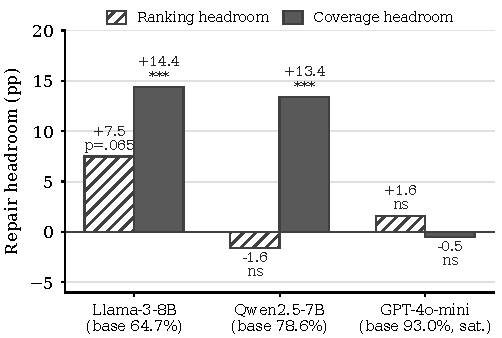
\includegraphics[width=\columnwidth]{../figures/decomposition.pdf}
\caption{Coverage headroom (planted $-$ \oraclecorpus) dwarfs ranking
headroom (\oraclecorpus $-$ base) on both non-saturated models and vanishes
on the saturated control. $^{***}$: $p{<}0.001$, exact McNemar.}
\label{fig:decomposition}
\end{figure}

\begin{table}[!t]
\caption{Coverage-vs-ranking decomposition ($n{=}187$; exact McNemar vs
baseline).}
\label{tab:decomposition}
\centering
\begin{tabular}{lrrrr}
\toprule
Model (base) & \oraclecorpus & planted & rank.\ hr & cov.\ hr \\
\midrule
Llama-3-8B (64.7\%) & 72.2\% & 86.6\% & $+7.5$ & $\mathbf{+14.4}$ \\
Qwen2.5-7B (78.6\%) & 77.0\% & 90.4\% & $-1.6$ & $\mathbf{+13.4}$ \\
GPT-4o-mini (93.0\%) & 94.7\% & 94.1\% & $+1.6$ & $-0.5$ \\
\bottomrule
\end{tabular}
\end{table}

Table~\ref{tab:decomposition} and Fig.~\ref{fig:decomposition} give the
central result. With a perfect example present, repair jumps $+21.9\pp$
(Llama-3-8B, $p{<}0.0001$). Decomposed, \textbf{coverage headroom is large
and significant on both non-saturated models} ($+14.4$, $+13.4\pp$;
$p{<}0.001$) and zero on the saturated control, while \textbf{ranking
headroom is small and heterogeneous} ($+7.5\pp$, $p{=}0.065$ on Llama;
$-1.6\pp$, ns, on Qwen --- forcing the best real example does not help). We
refuse to average these: the binding constraint is \emph{primarily corpus
coverage}. Most damaging for reranking: with the perfect example present,
plain dense retrieval surfaces it in the top-$k$ \emph{100\%} of the time;
\structured demotes it in 11/187 cases (94.1\%), with identical conversion
(86.6\% both). At the instance level, retrieval flips 37 of the 8B outcomes
(18 wins, 19 losses) and the mean retrieved-example relevance of wins
(2.645) is indistinguishable from losses (2.621). (\textsc{oracle\_self} ---
showing the model its own fix pattern --- reaches 90.4\%, $+25.7\pp$: a
sanity check that the model can exploit a near-identical example, not a
deployable ceiling.)

\subsection{RQ4: Transfer to real repository bugs --- unconfirmed}
\label{sec:results-transfer}

Synthetic mutations make perfect examples constructible by design, so RQ3
could be a synthetic-regime artifact. We test transfer end-to-end on real
PyBugHive bugs. First, with the project-held-out corpus, retrieval is
exactly neutral on \texttt{black} (baseline, \codeonly, \structured all
23/34), consistent with RQ2. Second, an initial single-project planted
pilot was encouraging: planting the exact buggy$\to$fixed pairs lifted
GPT-4o-mini from $85.7\%$ to $96.4\%$ on 28 black cases, converting all
four baseline failures ($b{=}1$, $c{=}4$, $p{=}0.375$, underpowered).

\begin{table}[!t]
\caption{Real-bug replication (PyBugHive, GPT-4o-mini, 55 cases usable in
all arms; exact McNemar vs baseline within one CI run).}
\label{tab:powered}
\centering
\begin{tabular}{lrrr}
\toprule
 & baseline & \structured(normal) & \structured(planted) \\
\midrule
pooled (55) & 42 (76.4\%) & 39 (70.9\%) & 39 (70.9\%) \\
\quad vs baseline & --- & $b{=}7$, $c{=}4$ & $b{=}7$, $c{=}4$ \\
\quad exact $p$ & --- & 0.549 & 0.549 \\
\midrule
black (26) & 23 & 20 & 23 \\
pandas (23) & 15 & 15 & 12 \\
other (6) & 4 & 4 & 4 \\
\bottomrule
\end{tabular}
\end{table}

The replication across every supported case (116 attempted, 55 usable;
Table~\ref{tab:powered}) \textbf{does not confirm the transfer}: planting
the exact fix pair yields $70.9\%$ vs baseline $76.4\%$ --- 4 baseline
failures converted, 7 passes regressed, $p{=}0.549$, 95\%~CI on the
difference $[-17.2, +6.3]\pp$. That interval \emph{excludes the pilot's
$+10.7\pp$ effect}, which is the replication's one firm conclusion; at the
observed discordance the design's MDE is ${\sim}16\pp$, so small effects in
either direction remain undetectable, and we do not claim a confirmed
null. Three observations bound the interpretation further. (i)~The pilot
itself did not reproduce: on the overlapping CI case set, black scores
23/26 in baseline and planted alike --- cross-environment variation of the
same magnitude as the arm differences, which is why we compare arms only
within the run. (ii)~Per-project effects are inconsistent (planting
matches baseline on black but costs three pandas cases), and the usable
set is 89\% black+pandas after project-correlated attrition
(Section~\ref{sec:design}), so the pooled estimate inherits that skew.
(iii)~The planted-vs-baseline contrast confounds any coverage benefit with
retrieval-prompt overhead, so we also report the clean coverage contrast:
planted vs \structured(normal), identical prompt shape, corpora differing
only in the plants. It is an exactly balanced null --- 10 discordant cases,
5 in each direction ($p{=}1.0$) --- i.e., with the pipeline held fixed,
adding the exact fix pairs to the corpus produced symmetric case churn and
zero net effect. An instrumented rerun explains part of why: \emph{the
planted pair reached the $k{=}2$ prompt in only 76\% of cases} (black:
65\%) --- near-duplicate plants from sibling bugs in the same large file
collide, and the reranker selects a different bug's pair (the
repository-scale form of the demotion effect in RQ3). So ``guaranteed''
corpus coverage does not guarantee \emph{prompt} coverage on real bugs.
Conversion also fails outright: all 7 regressions had applied patches that
failed tests (in the instrumented rerun, every regressed case \emph{did}
receive its planted pair), so an exact-fix example in the prompt neither
protects passing cases nor reliably converts failing ones. Table~\ref{tab:discordant} lists the 11 discordant baseline-vs-planted
cases with their retrieval status from the instrumented rerun.

\begin{table}[!t]
\caption{The 11 discordant baseline-vs-planted real-bug cases. ``Pair in
prompt'' from the instrumented rerun (retrieval-order nondeterminism may
differ per run). All regressions were applied patches that failed tests.}
\label{tab:discordant}
\centering
\small
\begin{tabular}{llll}
\toprule
Case & Outcome & Pair in prompt & Note \\
\midrule
black-232 & converted & no (sibling 297) & also converted in pilot \\
black-273 & converted & no (sibling 297) & also converted in pilot \\
black-297 & converted & yes & also converted in pilot \\
pandas-14973 & converted & yes & \\
black-95 & regressed & yes & applied, tests fail \\
black-238 & regressed & yes & applied, tests fail \\
black-334 & regressed & yes & applied, tests fail \\
pandas-14652 & regressed & yes & applied, tests fail \\
pandas-14770 & regressed & yes & applied, tests fail \\
pandas-14776 & regressed & yes & applied, tests fail \\
pandas-15488 & regressed & yes & applied, tests fail \\
\bottomrule
\end{tabular}
\end{table}

Two of the four conversions occurred \emph{without} the case's own pair in
the prompt (a sibling bug's pair from the same file was retrieved instead),
while every regression occurred \emph{with} it: whatever converts real bugs
here is not the exact-pair signal the coverage hypothesis posits.
What the replication establishes is therefore modest but real:
the encouraging single-project effect was not recovered at scale, and any
true pooled effect of guaranteed coverage on these real bugs is bounded
below $+6.3\pp$ --- far from the $+14$--$22\pp$ the synthetic
decomposition would predict.

\section{Discussion}
\label{sec:discussion}

\textbf{Why doesn't relevance convert?} A retrieved example helps only if it
is \emph{sufficiently} relevant to the specific fix, and realistic corpora
rarely contain such an example. When one exists (planted), even plain dense
retrieval finds it and repair converts; when none exists, improving the
\emph{ordering} of insufficient examples cannot manufacture the missing
knowledge. Headroom scales with the fraction of currently-failed problems a
perfect example would fix: $+14$/$+13\pp$ on the two mid-base-accuracy
models, ${\sim}0$ on the saturated one.

\textbf{Cost.} Measured on HumanEvalFix GPT-4o traces, the structured
prompt averages ${\sim}4\times$ the baseline's input tokens
(${\sim}1{,}158$ vs ${\sim}300$) plus embedding/index/retrieval
infrastructure, for equal-or-worse accuracy --- Pareto-dominated. The
actionable guidance follows from RQ3 and RQ4 together: reranking
sophistication has negative ROI everywhere we measured; corpus coverage is
where the headroom lives on synthetic bugs, so it is the better investment
--- but RQ4 cautions that on real repository bugs coverage alone does not
convert, and the patch-application and validation layers deserve the
attention that retrieval scoring currently gets.

\textbf{Evaluation hygiene.} Contamination can masquerade as retrieval
gains: an uncontrolled corpus (same-project entries) flipped our PyBugHive
results from neutral to strongly RAG-negative before the held-out control.
RAG-repair evaluations should hold out same-project corpus entries, ablate
post-processing separately from retrieval, and report equivalence bounds
rather than bare non-significance.

\textbf{Actionable insights.} For practitioners building single-shot
LLM repair: (i)~do not budget for retrieval reranking --- across six models
and four benchmarks it never paid off and cost ${\sim}4\times$ input tokens;
(ii)~if retrieval is used at all, plain dense retrieval over buggy code is
as good as any variant we built; (iii)~on benchmark-shaped bugs, corpus
coverage is the only retrieval lever with measurable headroom, and it is
worth curating; (iv)~on repository bugs, first instrument whether relevant
examples reach the prompt at all --- ours did only 76\% of the time under
near-duplicate collisions --- and invest in patch application and
validation before retrieval quality. For evaluators: (v)~hold out
same-project corpus entries; (vi)~report equivalence bounds and MDEs with
every null; (vii)~measure a cross-run noise floor before interpreting
small paired differences on real bugs; (viii)~never compare traced and
untraced runs' pass rates --- enabling tracing changed our pipeline's
patch-fallback behavior, an observer effect we caught only by diffing runs.

\section{Threats to Validity}
\label{sec:threats}

\emph{External validity:} the coverage decomposition
(RQ3) is established on synthetic mutations, where a ``perfect example'' is
constructible by design; the real-bug replication (RQ4) could not confirm
transfer, and that result is itself bounded --- 55/116 cases evaluable
after project-correlated attrition, a usable set dominated by two projects,
one model (GPT-4o-mini), and cross-environment variation: the local pilot
did not reproduce in CI, and a repeated instrumented CI run bounds
cross-run flips at 4--8\% of cases per arm --- comparable to the arm
differences themselves. \emph{Construct validity:}
both automated relevance measures are proxies sharing the retrieval
encoder; the \oraclecorpus\ arm selects the ``best real example'' by that
same proxy, so ranking headroom is underestimated to the extent the proxy
errs --- an asymmetry that would shift the decomposition toward ranking,
not away from coverage. The audit is weak corroboration only
(Section~\ref{sec:results}). The real-bug retrieval hit rate (76\%) was
measured in a separate instrumented rerun, not in the replication run
itself; retrieval-order nondeterminism in near-duplicate tie clusters
means per-case hit status may differ slightly between runs.
\emph{Internal validity:} the decomposition is one bug family, two
non-saturated models plus a saturated control; direction replicates across
architectures, magnitudes are benchmark-specific. \emph{Scope:} all
conclusions are bounded to single-shot, temperature-0, single-candidate,
$k{=}2$ pipelines; iterative and agentic regimes
(Section~\ref{sec:related}) may convert retrieval differently.
\emph{Power:} MDEs are $4.8$--$9.1\pp$ on the synthetic benchmarks and
${\sim}16\pp$ on the real-bug replication; equivalence claims are bounded
at $\pm 10\pp$.

\section{Artifact Availability}
\label{sec:artifact}

All code (retrieval pipeline, reranker, patch layer, evaluation harnesses),
corpus-construction scripts, the CI workflow for the real-bug replication,
per-case results for every reported run, the blind-audit worksheets and
scorer, and every analysis script (significance, equivalence/MDE,
independent relevance, oracle/planted decomposition) are provided as an
anonymized replication package: ANONYMIZED-ARTIFACT-URL. Retrieval corpora
and FAISS indexes are rebuilt from committed fixtures by the included
scripts. LLM outputs depend on closed-source APIs; we therefore ship the
cached per-case outputs so every number can be recomputed without API
access.

\section{Conclusion}
\label{sec:conclusion}

We set out to make retrieval-augmented repair work better by making
retrieval more relevant, and instead produced a cautionary decomposition of
why that framing fails. Structured failure-aware reranking can improve a
relevance proxy, but the gain is fragile across benchmarks, and even where
it holds it does not convert to significantly better repair in any of our
comparisons. On synthetic bugs, a planted-corpus experiment locates the
binding constraint in corpus coverage --- when a sufficiently relevant
example exists, plain dense retrieval already surfaces it and repair
improves by double digits; when it does not, no reranking sophistication
helps. On real repository bugs, our replication could not confirm that the
coverage effect transfers: planting exact fix pairs was
null-to-slightly-negative pooled ($p{=}0.55$), the confidence interval
excludes our own pilot's effect size, and effects below ${\sim}16\pp$
remain beyond the design's reach --- so we report transfer as
unestablished, with the diagnosis of the discordant cases as the key open
question. For practitioners working with single-shot repair pipelines: the
scorer is not the lever; the corpus is the lever on benchmark-shaped bugs;
and on real bugs the repair pipeline downstream of retrieval --- patch
application, localization, validation --- is where the evidence says
attention should go. Artifacts are described in Section~\ref{sec:artifact}.

\bibliographystyle{IEEEtran}
\bibliography{../references}

\end{document}
